\section{Analysis}\label{sec:analysis}

Building up on our initial idea and problem formulation, we determine two major functional areas that must be supported by our proposed system:

\begin{itemize}[noitemsep]
    \item \textit{\acrfull{pacs}} (access to restricted premises in a company or institution, building access control etc.)
    \item \textit{Online Access Control} (access to computer systems, applications, online sign-in etc.)
\end{itemize}

While the  typical question in a \acrshort{pacs} would be ``\textit{Is the person allowed to enter beyond this point}?'', and can be controlled by a variety of physical barriers, doors, turnstiles and the like, the online access control is more complex. Enterprises nowadays operate a wide spectrum of software solutions including on-premise applications, legacy systems, cloud-based and \acrshort{saas} applications, internally or externally oriented \acrshort{api}s and databases. All of these require some level of access control. To break down this structure, we first begin by identifying two service classes:
\begin{enumerate*}[label=(\roman*)]
    \item \textit{internal applications}, that sit within the enterprise security realm; and 
    \item \textit{external applications}, that include cloud based software, \acrshort{saas} solutions and partner/vendor applications, and which reside outside the given security realm.
\end{enumerate*}

The external applications can be further divided based on their interactions with the internal systems. Applications that are not business critical and/or are not integrated with the business processes may not require access to protected resources at all. Examples of such applications would be a lunch booking system or a company social network. These would be primarily used by the employees, but would not require connectors to business-critical systems and could therefore reside outside the security realm.

Other external applications, however, may require access to business-critical resources to function. \acrlong{crm} or payroll system may both be purchased as a \acrshort{saas}, but both require connectors to the protected resources to properly fulfil their functions. We can therefore extend our classification of the external applications accordingly -- applications that
\begin{enumerate*}[label=(\roman*)]
    \item \textit{require access to protected resources} and
    \item \textit{do not require access to protected resources}.
\end{enumerate*}
% TODO MAybe add stuff about user protected resources and Enterprise protected resources.

The access control of \textit{internal applications} will likely differ from access control of \textit{external applications} and similarly, the access control for applications that require access to protected resource will differ from those that do not. We can therefore devise an access control breakdown chart, as shown in Figure~\ref{fig:acs-classification}. 

Multiple sources list Identification, Authentication and Authorisation as the three basic steps in access control~\cite{Harris2008CISSPGuide, 2018AccessSystems, 2003IdentificationAuthorization}. We focus on authentication and authorisation in the system design and describe these further in the following sections.

\begin{figure}[ht]
    \centering
    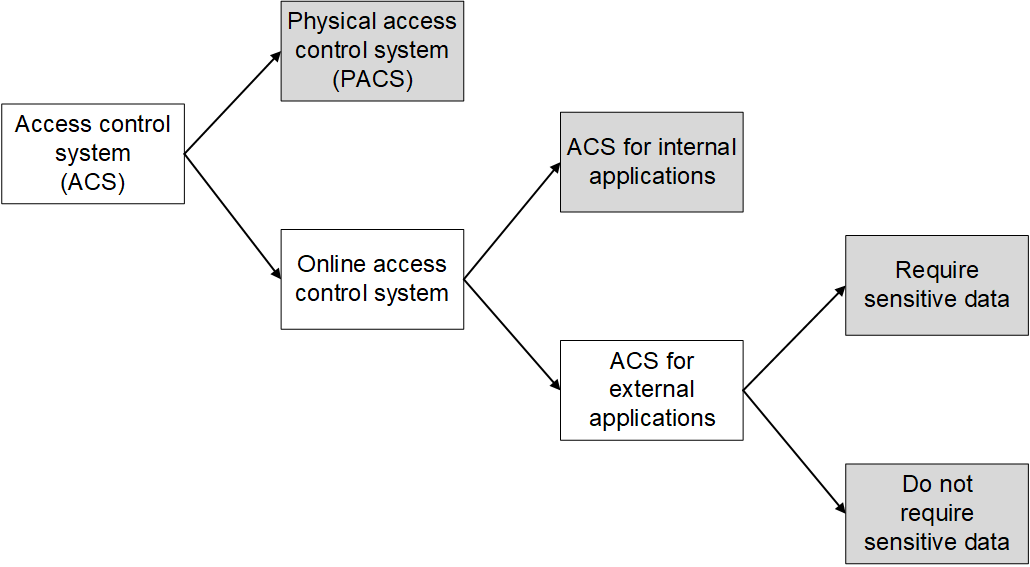
\includegraphics[width=.95\textwidth]{acs-classification}
    \caption{Access control system breakdown chart. \acrshort{acs} for external applications is different for applications that work with sensitive data from \acrshort{acs} and for external applications that do not work with sensitive data.}
    \label{fig:acs-classification}
\end{figure}

\subsection{Authentication}\label{sec:analysis-authentication}
In \acrshort{pacs}, physical tokens, such as ID cards, are the common practice nowadays. A survey carried out in 2016 indicated that above 40\% of the companies use low frequency proximity cards as their main method for personal authentication~\cite{HIDGlobal2017TheEnterprise}. These cards, operating in 125-134kHz frequency range are considered an obsolete technology and are not secure~\cite{Hakamaki2015SecurityTechnology}. On the other hand, around 20\% of the companies indicated use of mobile devices as a part of their \acrshort{pacs} solution~\cite{HIDGlobal2017TheEnterprise}. 

The main benefit of using a mobile device for this purpose is, that most people already own a smartphone and usually carry it with them at all times. Other technologies represented in the survey that are considered secure today, include iCLASS (contact-less card) and MIFARE DesFire (contact-less card). FIDO, nor FIDO2 keys (NFC, Bluetooth, or other) are not mentioned in the survey, although compatible \acrshort{pacs} systems exist on the market today\footnotemark. 

FIDO and FIDO2 enjoy support of big companies like Google, Facebook and Microsoft, but consumer-oriented services from these providers only permit the use of FIDO/FIDO2 as the second authentication factor. Google uses FIDO U2F keys for their employees, but only as a password replacement in the online login scenario~\cite{Krebs2018Google:Phishing} and Microsoft only supports FIDO2 keys with personal Microsoft accounts. As shown in Section~\ref{sec:online-access-control}, even Azure AD does not support this technology. To explore how FIDO2 can be used for hybrid access control on an enterprise scale, we propose the support of FIDO2 as a requirement for our system.
% 
\footnotetext{\url{https://web.archive.org/web/20190319221618/https://www.yubico.com/works-with-yubikey/catalog/modis/}, accessed 19 March 2019}

There is already a variety of devices that have been FIDO2 certified, with the Android system being a recent addition to the list~\cite{FIDOAlliance2019AndroidPasswords}. Considerations need to be put into how the FIDO2 flow is incorporated in the system and which of the FIDO2-certified devices are used in the flow. In the \acrshort{pacs} usability, namely the speed, is an important criteria, since existing systems already offer very low- to no-latency during a typical door opening use case. Beyond \acrshort{pacs}, the current access control solutions are mostly used for employee identification (as an ID badge)~\cite{HIDGlobal2017TheEnterprise} and the employee is only issued a single badge. The recommended approach in case the employee forgets the badge is to assign a temporary one that can be used during a limited time period and must be returned afterwards~\cite{Ryan2018HowBadges}.

In the online authentication, we can see that the systems support a wider range of authentication (and account recovery) methods, and the user is left to decide, which is authentication method do they prefer (see Section~\ref{sec:online-access-control}). Offering multiple methods simultaneously makes sense in the online access control scenario, because unlike in \acrshort{pacs}, where the on-site reception/security personnel can verify employees' identity and issue a temporary badge, in the online access control the identity verification is more complicated. In the case of forgotten credentials, the identity would therefore needed to be verified remotely (typically over phone), which is not feasible.

In the proposed hybrid access control system, it is desired to provide an authenticator, that is both fast to use and can be easily complemented and/or substituted with another authentication method if lost or forgotten. We propose the combination of FIDO2 key with \acrshort{nfc} as the primary authenticator, and FIDO2 enabled smartphone as the supplementary authenticator to meet the above criteria. The FIDO2 key with NFC support offers proximity-card-like usability (the user needs to swipe/hold the key next to the reader). If lost or forgotten, it can be substituted by an FIDO2 enabled smartphone, as people generally carry a smartphone with them, while at work. During our research, we have not encountered systems which offer the same selection of technologies, although the combination of a smartphone and an access card was seen in Section~\ref{sec:pacs-hid}.

% TODO FIDO2 would be used for all 4 boxes from access control breakdown chart

% TODO How OpenID connect is used for authentication/SSO
% TODO What information needs to be shared (Default OIDC scope - name, email, UID)...?
% TODO What entities will be needed (OID provider)
% TODO OpenID connect would be used only for boxes 3 and 4 from access control breakdown chart


% For \acrlong{aal}s 2 and 3 defined in 
% %  REFERENCE SECURITY REQUIREMENTS FOR CRYPTOGRAPHIC MODULES
% , authentication must be carried out using at least two independent factors. This requirement, together with abandonment of memorised secrets results in adoption of new authenticators. These  authenticators should offer at better security as memorised secrets, while maintaining the same level of accessibility. In 

\subsection{Authorisation}

When someone is authorise to use a system, it means they have permission to access that system. However, in enterprise access control scenario, there are other concepts associated with authorisation, rather than only verifying whether a user is allowed to use a certain system. The support for federated identity and the ability to handle \acrfull{sso} are typically design parameters that fall under the broader authorisation scope. Technologies that support these are discussed in the following section.

We can assume that an enterprise operates a variety of different IT systems, some of which may operate within the enterprise's security realm, while others may be \acrshort{saas} or may be operated by a business partner. To avoid an employee needing to manage several sets of credentials (one set for each system), federated identity is used. The access control system in an enterprise needs to be able to integrate with business application, so that federated identity can be used to access applications throughout the application landscape.

Once we acknowledge that a user should be able to use a single account (i.e. one set of credentials) to log in to both internal and external applications, we should further aim to reduce the number of times these credentials need to be entered, as the user logs into different systems, but without compromising the security of these systems. Single sign on addresses this need. With the single sign on, we could for example specify, that the user only needs to authenticate with their credentials once per two hours on a single machine. Once the user has authenticated, all the following requests to log in to any application using user's federated identity will be carried out without prompting the user to authenticate again, until the time limit has expired. This increases the convenience for the user.

Several technologies on the market support this approach. The most prominent ones, which we consider further are \acrshort{saml} and the OAuth + \acrshort{oidc} combination. Business applications that support federated identity integration, tend to support at least one of these technologies. While we could not find statistics comparing the use of the two in enterprises, we found examples of applications supporting both \acrshort{saml} and OAuth + \acrshort{oidc} and examples of applications that only support \acrshort{saml} (see Appendix~\ref{sec:appendix-links} for details). 

By some, \acrshort{saml} is considered as the enterprise-oriented technology, while OAuth and \acrshort{oidc} are considered oriented on the consumer market~\cite{Fagbemi2016ComparingWS-Federation, SoftwareSecured2016Differentiating2, OneLoginInc.SAMLOAuth}. However, OAuth and \acrshort{oidc} have been published 7 and 9 years  (respectively) after \acrshort{saml}. It is therefore understandable, that \acrshort{saml} is still widely present in the enterprise market. However, both technologies can be used in an enterprise environment, as noted by~\cite{Naik2017SecuringConnect} and some even encourage the use of OAuth + \acrshort{oidc} as the preferred way for new applications~\cite{barbkess2019SingleDirectory}.

Advantages of \acrshort{saml} include speed, identity-provider-initiated \acrshort{sso} and wide adoption~\cite{OneLoginInc.SAMLOAuth, Naik2017SecuringConnect}. The weaknesses are the limited support for mobile/native applications and heavy weight of the protocol (due to XML)~\cite{Naik2017SecuringConnect}. Conversely, the advantages of OAuth in combination with \acrshort{oidc} include better support for mobile and native applications, and more light-weight and REST-friendly protocol~\cite{Naik2017SecuringConnect}. There exists a proposal to improve the speed of OAuth in an enterprise setting~\cite{Noureddine2011AEnterprise}.

Because of better suitability for mobile and native applications, we propose OAuth + \acrshort{oidc} as the primary choice of authorisation and \acrshort{sso} protocols for internal enterprise applications and for external applications that support these technologies. Naturally, the system is likely to be integrated with internal legacy applications and external applications that do not support OAuth + \acrshort{oidc} for \acrshort{sso}. While a solution was proposed to enable OAuth functionality on legacy systems via \acrfull{esb}, this is not yet widely adopted and requires integration of an \acrshort{esb}~\cite{deSousaRibeiro2018AnBus}. Therefore the system should also support the \acrshort{saml} flow to accommodate these legacy systems.



% maybe-TODO Which scopes need to be included
% maybe-TODO Which entities will be needed to support this (Authorisation server)

% maybe-TODO OAuth will be used for boxes 3 and 4 from access control breakdown chart
\subsection{Access Policy Management}\label{Access_Policy_Management_Analysis}

In every \acrlong{acs}, the model used for granting the access play a crucial role as the system is dependent on it. Often it makes it easier for the administrator to manage and grant the access to employees, but if wrong model is chosen or is wrongly implemented, it can make the work even more burdensome. As it was outlined in the State of the Art (Chapter \ref{SOTA}), we are looking into \acrshort{rbac} and \acrshort{abac} as models for Identity and Access Management as they are the most used ones these days~\cite{2018BestV3}.

Both models offer a range of functionality and suits specific enterprises. One of \acrshort{rbac}’s big advantages is the ease of creating and maintaining the roles and system as a whole, but as the enterprise grows and more roles and resources are introduced, it gets complicated and hard to have an overview. Therefore, \acrshort{rbac} is suitable for small to medium enterprises. It is less complex than \acrshort{abac} and therefore it offers low level of granularity. Permission only can be granted to roles, not to operations or objects. On-the-fly contextual decisions are not supported, as well as restrictions can only be applied to parts of the system, not on specific data. Also, only known parameters can be used during implementation and environmental restrictions cannot be implemented. Even though, \acrshort{rbac} is older model it still offers adequate functionality.

On the other hand, \acrshort{abac} model which is based on attributes and policies presents fine grain and multi-dimensional access control. Biggest advantages of \acrshort{abac} over \acrshort{rbac} are the scalability of the model, dynamic parameters, easy maintenance and support for on-the-fly context aware decisions as information about requesting subject, requested object and environmental attributes are present. This way it is possible to grant access to specific data at specific times based on location. Initial configuration of the system is more complex compared to \acrshort{rbac}, but once done, it is easy to add new attributes or policies which are automatically executed. 

As the focus of the project, is to offer \acrlong{acs} to big enterprises, allowing fine grain control over resources, \acrlong{abac} model is more suitable for the solution. The trend in the industry is to adopt \acrshort{abac} more and more, and Gartner predicts that \textit{``By 2020, 70\% of businesses will use attribute-based access control (\acrshort{abac}) to protect critical assets''}~\cite{GartnerGartnerPredictions}. Studies also shows, that \acrshort{abac} is the model which should be used by enterprises in the future, rather than \acrshort{rbac}~\cite{Fatima2016TowardsArgument}.

To implement \acrshort{abac} model, the standard have to chosen as well. The most wide-spread standard is \acrshort{xacml}, which is explained in Section \ref{sec:xacml}, but others such as \acrfull{alfa} or \acrfull{ngac} exists as well. \acrshort{alfa} is a pseudocode language based on \acrshort{xacml} which provide higher user-friendliness, lower complexity and overall similar performance~\cite{Mejri2016FormalPolicies}. \acrshort{ngac} on the other hand, even-though it uses \acrshort{abac} model for access control, its implementation differs from \acrshort{xacml}~\cite{Ferraiolo2016ANGAC}. For the purpose of this project, we decide and propose the use of \acrshort{xacml} as the standard for implementing \acrshort{abac} in the system, mainly because of its wide spread, similar functionality to \acrshort{ngac} and the fact that it is being taught at the Identity and Access Management course at the university.
\subsection{Use Cases} \label{sec:analysis-usecases}
Use cases are a valuable analysis technique for obtaining requirements subsequently. They represent actions of actors (humans, external systems) which can be performed within the system in order to achieve a goal. 

% TODO possible reference here: "Writing effective use cases"

The first step when creating a use case is to identify all actors that are interacting with the system. Our primary actor is the user -- an employee of an enterprise who is using the system to sign-in to a service or get through a physical checkpoint. The employee should also be able to carry out basic administrative tasks on their own account, such as revoke a lost or stolen authenticator, set up additional authenticators, such as smartphones, to increase convenience (provided that the enterprise policy permits the use of such),  and set up account recovery methods, such as security questions, or one-time passwords.
% TODO Add reference to previous discussion (should be within Analysis or SOTA).

Another actor in our system is the administrator. The administrator manages employees and their enterprise digital identities within the \acrshort{acs}, as well as the attributes and policies for accessing resources. Furthermore, the administrator sets-up and manages connections with external business systems (external clients). The right side of the diagram shows the receiving actors: these are the internal systems and external systems, which the employees require access to, and which may need to manipulate employee's protected resources during their operation. Additionally, the external systems may also require access to enterprise protected resources (protected resources, which are not bound to a single user), as discussed previously\footnotemark.
% TODO Add reference to previous discussion (should be within Analysis).
% 
\footnotetext{Internal systems might also require access to protected resources for their operation. However, it is assumed that internal systems can access the protected resource directly, without intervention from the \acrshort{acs}.}

Having the knowledge of the actors interacting with the system and their primary actions, we can identify the following set of use cases (list in figure~\ref{fig:use-cases-list}). 

\begin{figure}[H]
    \centering
    \begin{multicols}{2}
    \begin{enumerate}[noitemsep,nolistsep]
        \item[UC-1] Sign-in to a service
        \item[UC-2] Pass through a physical checkpoint
        \item[UC-3] Manage account security
        \item[UC-4] Revoke an authenticator
        \item[UC-5] Register additional authenticator
        \item[UC-6] Set-up an account recovery method
        \item[UC-7] Manage users
        \item[UC-8] Add user
        \item[UC-9] Remove user
        \item[UC-10] Modify user attributes
        \item[UC-11] Manage policies
        \item[UC-12] Add policy
        \item[UC-13] Modify policy
        \item[UC-14] Remove policy
        \item[UC-15] Manage client connections
        \item[UC-16] Access protected resources
        \item[UC-17] Access user protected resources
        \item[UC-18] Access enterprise protected resources
    \end{enumerate}
    \end{multicols}
    \caption{List of use cases for the proposed \acrshort{acs}. Some use cases are a generalisation of other, more granular items. For example UC-11 is a generalisation of UC-12, UC-13 and UC-14. Figure~\ref{fig:use-case-diagram} shows these generalisations.}
    \label{fig:use-cases-list}
\end{figure}

In total eighteen use cases are identified as shown above. Figure~\ref{fig:use-case-diagram} in Appendix~\ref{sec:use-case-diagram} on page~\pageref{fig:use-case-diagram} illustrates the composition of these use cases and the relationships between actors and the use cases. The proposed system should cater to all of these use cases, as they are all necessary for the system to be deployable in an enterprise scenario. More functionality could be added to the system, introducing further use cases and richer interactions. However, this functionality is beyond the \acrlong{mvp} and is not listed here.

% First two use cases come from the basis of this project, which tries to solve the access of employees to protected resources both online and on premise (\acrshort{uc}-1, 2). Once having an authenticator, it is vital to have a way to revoke it, in case it has been stolen or compromised (\acrshort{uc}-3). Adding additional authenticator is crucial for implementation of the system in highly secure facilities, where authentication with only one factor may not be enough (\acrshort{uc}-4). Following, if all authenticators are compromised, there should be a way of recovering the enterprise digital identity, therefore, adding a recovery method is essential (\acrshort{uc}-5). In order to keep the system updated and maintained, there should be a way of managing everything, that is the role of administrator who needs to be able to manage employees (\acrshort{uc}-6), manage their attributed so they can access various resources (\acrshort{uc}-7), manage the policies which determine who can access resources (\acrshort{uc}-8) and manage connections with external clients (\acrshort{uc}-9). Lastly, protected resources needs to be made available for systems, both internal and external, so they can function properly (\acrshort{uc}-10).
\subsection{Requirements} \label{sec:analysis-requirements}
The following section describes the requirements of the proposed system. The requirements have been derived based on the analysis in previous sections of this chapter. Two kinds of requirements are presented -- the functional requirements and non-functional requirements. 

The requirements listed here are proposed as the necessary requirements for the deployment of the system into production (\acrlong{mvp}). As discussed in the Use Cases section, a fully mature system could introduce many more functional requirements, however these are not listed here. Because all the listed requirements are necessary for the operation of the system, they all must be implemented in an \acrshort{mvp} and therefore no prioritisation method is used. The additional possible functionalities of the system are discussed in Section~\ref{sec:discussion} (p.~\pageref{sec:discussion}).

\subsubsection{Functional Requirements} \label{sec:analysis-functionalReqruiements}
Functional requirements describe what does the system do and which features does it have. Table~\ref{tab:functional-requirements} (p.~\pageref{tab:functional-requirements}) lists these requirements for the proposed system. The \textit{Reference} column indicates the origin of the given requirement to map, why that requirement has been included.

% NOTE: Moved tha whole table to a new file (was getting too big and was in the way).
\subsubsection{Non-functional requirements} \label{sec:analysis-nonfunctional}
Non-functional requirements describe how the system is and how does it perform. They can be evaluated based on measures~\cite{Adams2015NonfunctionalDesign}. User usually does not directly see their implementation, but can rather feel it by the system performance. Often they influence the architecture of the system. Table~\ref{tab:nonfunctional-requirements} lists these requirements for the proposed system. The \textit{Reference} column indicates the origin of the given requirement to map, why that requirement has been included.

\bigskip\noindent
In this chapter we first define four categories of access control problems. We continue by considering the access control problem and possible solutions from the perspectives of authentication, authorisation and access policies. We then identify the basic use cases of a combined access control system and use these to derive the functional and non-functional requirements. In the next chapter we describe the design of the system in greater detail.
\newgeometry{left=1.2cm,right=1.2cm,top=2cm,bottom=2cm,footskip=.8cm}
\begin{table}[htbp!]
    \footnotesize
    \onehalfspacing
    \centering
    \begin{tabular}{|c|p{15cm}|c|}
    \hline
    \cellcolor[HTML]{CBCEFB}\textbf{ID}&\cellcolor[HTML]{CBCEFB}\textbf{Description}&\cellcolor[HTML]{CBCEFB}\textbf{Reference}\\
    \hline
    RQ-1&User must be able to authenticate with a single-factor cryptographic device based on FIDO2 to use their enterprise digital identity.&Section~\ref{sec:analysis-authentication}\\
    \hline
    RQ-2&User must be able to authenticate with a smartphone, using FIDO2 to use their enterprise digital identity.&Section~\ref{sec:analysis-authentication}\\
    \hline
    \hline
    RQ-3&User must be able to sign-in to an internal system with their enterprise digital identity.&\makecell{Section~\ref{sec:analysis-authorisation}\\and UC-1}\\
    \hline
    RQ-4&User must be able to sign-in to an external client system with their enterprise digital identity.&\makecell{Section~\ref{sec:analysis-authorisation}\\ and UC-1}\\
    \hline
    \hline
    RQ-5&User must be able to pass through a physical checkpoint with their enterprise digital identity.&UC-2\\
    \hline
    \hline
    RQ-6&User must be able to revoke their authenticator.&UC-4\\
    \hline
    RQ-7&Administrator must be able to revoke user’s authenticator.&UC-4\\
    \hline
    \hline
    RQ-8&User must be able to register additional authenticator.&UC-5\\
    \hline
    RQ-9&Administrator must be able to register user’s authenticator.&UC-5\\
    \hline
    \hline
    RQ-10&User must be able to set-up account recovery (e.g. combination of OTP, phone call, e-mail).&UC-6\\
    \hline
    \hline
    RQ-11&Administrator must be able to create new enterprise digital identity.&UC-8\\
    \hline
    \hline
    RQ-12&Administrator must be able to delete enterprise digital identity.&UC-9\\
    \hline
    \hline
    RQ-13&Administrator must be able to modify attributes of users.&UC-10\\
    \hline
    \hline
    RQ-14&Administrator must be able to set-up a policy.&UC-12\\
    \hline
    RQ-15&Administrator must be able to modify a policy.&UC-13\\
    \hline
    RQ-16&Administrator must be able to delete a policy.&UC-14\\
    \hline
    \hline
    RQ-17&Administrator must be able to create new connections to external client systems.&UC-15\\
    \hline
    \hline
    RQ-18&External client system must be able to access protected resources if a permission was granted.&UC-16\\
    \hline
    RQ-19&External client system must be able to obtain a grant permission.&UC-16\\
    \hline
    \end{tabular}
    \caption{List of functional requirements for the \acrshort{mvp} with the reference to their origin.}
    \label{tab:functional-requirements}
\end{table}
% 
\begin{table}[htbp!]
    \footnotesize
    \onehalfspacing
    \centering
    \begin{tabular}{|c|p{15cm}|c|}
    \hline
    \cellcolor[HTML]{CBCEFB}\textbf{ID}&\cellcolor[HTML]{CBCEFB}\textbf{Description}&\cellcolor[HTML]{CBCEFB}\textbf{Reference}\\
    \hline
    RQ-20&Authentication to PACS using enterprise digital identity must be comparably fast to traditional RFID access cards (order of milliseconds to seconds).&\makecell{Section \ref{sec:analysis-authentication} \\ and UC-2}\\
    \hline
    RQ-21&The system must use OIDC + OAuth for Authentication and Authorisation.&\makecell{Section \ref{sec:analysis-authentication} \\ and \ref{sec:analysis-authorisation}}\\
    \hline
    RQ-22&The system must use XACML for access policy management.&Section \ref{sec:analysis-access-policy}\\
    \hline
    \end{tabular}
    \caption{List of non-functional requirements for the \acrshort{mvp} with the reference to where they are collected from.}
    \label{tab:nonfunctional-requirements}
\end{table}
\restoregeometry